\documentclass[a4paper,10pt]{report}

\usepackage[latin1]{inputenc}
\usepackage[T1]{fontenc}
\usepackage[english]{babel}
%\usepackage[osf,noBBpl]{mathpazo}
\usepackage{bold-extra}
\usepackage{euler}
\usepackage{enumitem}
\usepackage{mathrsfs, amsfonts, amssymb, amsmath, mathtools, amsthm, stmaryrd, graphicx, wrapfig, listings}
%\usepackage{color}
\usepackage{xcolor}
\usepackage{hyperref}
\usepackage{comment}
\usepackage{subcaption}
%\usepackage{pgfkeys}


%%%%%%%%%%%%%%%%%%%%%%%%%%%%%%%%%% Theorems et al., fix at some point %%%%%%%%%%%%%%%%%%%%%%%%%%%

\theoremstyle{plain}
\newtheorem{teo}{Theorem}[chapter]
\newtheorem*{teo*}{Theorem}
\newtheorem{prop}{Proposition}[chapter]
\newtheorem{claim}{Claim}[section]
\newtheorem{cor}{Corollary}[chapter]
\newtheorem{lema}{Lemma}

\theoremstyle{remark}
\newtheorem*{notation}{Notation}
\newtheorem{remark}{\textbf{\textit{Remark}}}[chapter]

\theoremstyle{plain}
\newtheorem{defn}{Definition}[chapter]
\newtheorem{obs}{Observation}
\newtheorem*{example}{Example}
\newtheorem*{excercise}{Excercise}

\newcommand*{\QED}{\hfill\ensuremath{\square}}%
\newcommand*{\QEDA}{\hfill\ensuremath{\blacksquare}}%
\newcommand*{\ext}{\mathrm{ext}}
\newcommand*{\extC}{\mathrm{extC}}


\renewcommand\proofname{\scshape \textit{Proof.} \normalfont}
\renewcommand{\labelitemi}{$\bullet$}
\renewcommand{\labelitemii}{$\star$}
\renewcommand{\labelitemiii}{$\diamond$}
\renewcommand{\labelitemiv}{$\ast$}

%%%%%%%%%%%%%%%%%%%%%%%%%%%%%%%%%% Theorems et al., fix at some point %%%%%%%%%%%%%%%%%%%%%%%%%%%

\title{Characterization of circle split graphs by minimal forbidden subgraphs}
\author{Nina Pardal}
\date{\today}

\definecolor{dark-blue}{RGB}{60,80,170}
\definecolor{dark-red}{RGB}{240,50,60}

\begin{document}

\chapter{Circle split graphs containing a tent}

\section{Nested and 2-nested matrices}

We begin by introducing some notation. Let $A$ be a $(0,1)$-matrix.
We define $a_{i,j}$ for $1 \leq i \leq n, 1 \leq j \leq m$, to the entry of $A$ in row $i$ and column $j$. 
We note $a_{.,j}$ to the column vector $j$ of the matrix $A$ and $a_{i,.}$ to the row vector $i$ of the matrix $A$.
	
We define $l_i = \min_{1 \leq j \leq m} \{ j \mid a_{i,j} = 1 \}$ and $r_i = \max_{1 \leq j \leq m} \{ j \mid a_{i,j} = 1 \}$.
	
We say that two rows $a_{i,.}$ and $a_{k,.}$ are disjoint, if there is no column index $1 \leq j \leq m$ such that $a_{i,j} = a_{k,j} = 1$.
We say that $a_{i,.}$ is nested (or included) in $a_{k,.}$ if, for every $1 \leq j \leq m$ such that $a_{i,j} = 1$, then $a_{k,j} = 1$.
	
Finally, we say that \emph{$a_{i,.}, a_{k,.}$ start (respectively end) in the same column} if $l_i = l_k$ (respectively $r_i = r_k$), 
and we say \emph{$a_{i,.}, a_{k,.}$ start (end) in different columns} if $l_i \neq l_k$ (respectively $r_i \neq r_k$).


\begin{defn} \label{def_nested_matrix}
	We say a $(0,1)$-matrix is \emph{nested} if it has the consecutive ones property for the rows 	($C1P$) and every two rows are either disjoint or nested.
\end{defn}

\begin{defn} \label{def_2nested_matrix}
	We say a $(0,1)$-matrix is \emph{$2$-nested} if it has the $C1P$ for the rows, 
	and there is a partition $S_1, S_2$ of the rows such that each submatrix
	obtained is nested.
\end{defn}

Tucker characterized all the minimal forbidden submatrices for the $C1P$. 
See Figure \ref{fig:tucker_matrices} for the complete list of Tucker matrices.

\begin{figure}[h!]
	\centering
	\begin{align*}
			M_I(k)&= \begin{pmatrix}
				110...00\\
				011...00\\
				.   .   .   .   . \\
				.   .   .   .   . \\
				.   .   .   .   . \\
				000...11\\
				100...01\\
			\end{pmatrix}
			&
			M_{II}(k)&= \begin{pmatrix}
				011...111\\
				110...000\\
				011...000\\
				.   .   .   .   . \\
				.   .   .   .   . \\
				000...110\\
				111...101\\
			\end{pmatrix}
			&
			M_{III}(k)&= \begin{pmatrix}
				110...000\\
				011...000\\
				.   .   .   .   . \\
				.   .   .   .   . \\
				000...110\\
				011...101\\
			\end{pmatrix}
			\\
			\end{align*}
			\begin{align*}
			M_{IV}&= \begin{pmatrix}
				110000\\
				001100\\
				000011\\
				010101\\
			\end{pmatrix}
			&
			M_{V}&= \begin{pmatrix}
				11000\\
				00110\\
				11110\\
				10011\\
			\end{pmatrix}
	\end{align*}
	\caption{Tucker matrices: $M_{I}(k) \in \{0,1\}^{k \times k}$, $M_{III}(k) \in \{0,1\}^{k \times k+1}$ with $k \geq 3$,
 	and $M_{II}(k) \in \{0,1\}^{k \times k}$ with $k \geq 4$}
\end{figure} \label{fig:tucker_matrices}

Let $G =(K,S)$ a split graph, where $n=|S|, m=|K|$ let $S=\{ s_1, \ldots, s_n \}$ and $K=\{ v_1, \ldots, v_m \}$ be an ordering of $S$ and $K$. 
Let $A= A(S,K)$ be the associated matrix of $n$ rows and $m$ columns such that 

\[ A\left( i,j \right) = \begin{cases} 
      1 & \mbox{ if } s_i \mbox{ is adjacent to } v_j \\
      0 & \mbox{ if } s_i \mbox{ is nonadjacent to } v_j  
   \end{cases}
\]

Thus the column $j$ of $A$ corresponds to the adjacency in $S$ of the vertex $v_j$.

Correspondingly, we define nested and $2$-nested graphs as follows.

\begin{defn} \label{def_nested}
	Let $G = (K,S)$ be a split graph with a linear ordering $\Pi$ of $K$. 
	$G$ is said to be \emph{nested} regarding $\Pi$ if the associated matrix $A(S,K)$ is nested.
\end{defn}

\begin{defn} \label{def_2nested}
		Let $G = (K,S)$ be a split graph with a linear ordering $\Pi$ of $K$. 
	$G$ is said to be \emph{nested} regarding $\Pi$ if the associated matrix $A(S,K)$ 
	is $2$-nested.
\end{defn}


\subsection{Nested matrices}

Let $A$ be a $(0,1)$-matrix. We define the auxiliary graph $H(A)=(V,E)$ where the vertex set $V= \{ w_1, \ldots, w_n \}$ has one vertex for each row in the matrix $A$, 
and two vertices $w_i,w_k \in V$ are adjacent if and only if the rows $a_{i,.}$ and $a_{k,.}$ are neither disjoint or nested.
	
When we refer to the vertex $w_i$, we will be speaking as needed in each case for abuse of language both of the vertex in $H(A)$ and the row array $a_{i,.}$ of $A$. 
Thus, the previous definitions apply to the vertices in $H(A)$:
we say two vertices $w_i$ and $w_k$ in $H(A)$ are nested (respectively disjoint) if the corresponding rows $a_{i,.}, a_{k,.}$ are nested (disjoint).
And two vertices $w_i, w_k$ in $H(A)$ start (end) in the same column if the corresponding rows $a_{i,.}, a_{k,.}$ start (end) in the same column.

\vspace{2mm}
Suppose that the $(0,1)-$matrix $A$ is nested. Since Tucker matrices (see Figure \ref{fig:tucker_matrices}) are \textit{all} the minimal forbidden submatrices for the C1P, 
thus the first condition of the definition of nested gives these matrices 
as forbidden submatrices.

Furthermore, the fact that every pair of rows are either disjoint or nested, implies that the gem matrix $G_0$ (see Figure \ref{fig:forb_nested}) is a forbidden submatrix of $A$,
for in this case, the two rows of the gem matrix are neither disjoint nor comparable.
This matrix also represents a gem subgraph in the associated graph $G$.
Moreover, observe that $G_0$ is the minimal submatrix with this property, and also every Tucker matrix has $G_0$ has a submatrix, thus $G_0$ is the only minimal submatrix for nested matrices.
The following result is an inmediate consequence of the latter.

\begin{teo}
	A $(0,1)$-matrix is nested if and only if it does not contain $G_0$ as a submatrix.
\end{teo}


\begin{figure}[h!]

	\centering  
	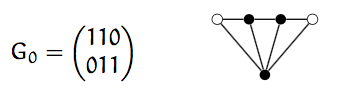
\includegraphics[scale=.6]{nested_forb.png}

	\caption{\mbox{The gem matrix } $G_0$ \mbox{, and the gem subgraph in the associated graph } $G$ \mbox{: black vertices are in} $K$ \mbox{and white vertices in }$S$}
	\label{fig:forb_nested}
\end{figure}

As a corolary, we have the following theorem for nested graphs.

\begin{teo}
	A split graph $G = (K,S)$ is nested if and only if it does not contain any gem as an induced subgraph.
\end{teo}

\subsection{2-nested matrices}

\begin{teo}
	A $(0,1)$-matrix $A$ is $2-$nested if and only if there is a linear ordering $\Pi$ of the columns such that the matrix $A$ with its column ordered according to $\Pi$ does not contain any Tucker matrix, or $F_0$, $F_1(k)$, $F_2(k)$ for $k \geq 5$ (see Figure \ref{fig:forb_B-A}) as submatrices.
\end{teo}

\begin{figure}[h!]
	\centering
	\begin{align*}
			F_0= \begin{pmatrix}
				11100\\
				01110\\
				00111\\
			\end{pmatrix}
			&&
			F_1(k)= \begin{pmatrix}
				011...111\\
				111...110\\
				000...011\\
				000...110\\
				.   .   .   .   . \\
				.   .   .   .   . \\
				.   .   .   .   . \\
				110...000\\
			\end{pmatrix}
			&&
			F_2(k)= \begin{pmatrix}
				0111...10\\
				1100...00\\
				0110...00\\
				.   .   .   .   . \\
				.   .   .   .   . \\
				.   .   .   .   . \\
				0000...11\\
			\end{pmatrix}
	\end{align*}
	\caption{The matrices $F_0$, $F_1(k) \in \{0,1\}^{k \times k-1}$, and $F_2(k) \in \{0,1\}^{k \times k}$, with $k \geq 5$.}
\end{figure}\label{fig:forb_B-A}

It follows from the definition of \ref{def_2nested}, that the existence of such partition for the rows of the matrix $A$ is equivalent to having a bicoloring of the auxiliary graph $H(A)$ defined before. Thus, is equivalent to asking $H(A)$ to be a bipartite graph. 
Recall that bipartite graphs have the odd chordless cycles as minimal forbidden induced subgraphs.

\begin{proof}
	$ \Leftarrow )$ Let $\Pi$ be a linear ordering of the columns such that the matrix $A$ does not contain any $F_0, F_1(k), F_2(k)$ or Tucker matrices as submatrices, for $k\geq 5$.
	
	Due to Tucker's Theorem, since there are no Tucker submatrices in $A$, we may assert that the matrix $A$ has the $C1P$ 
	and hence the first condition of the definition of $2-$nested holds.
	
	\vspace{.5mm}
	Toward a contradiction, suppose that even though $A$ has the $C1P$, the auxiliary graph $H(A)$ does not admit a bicoloring of its vertices.
	Thus, there is an induced odd cycle in $H(A)$. We will show that, depending on the length of the odd cycle, 
	we can find $F_0$, $F_1(k)$ or $F_2(k)$ as submatrices of $A$, and thus reaching a contradiction.

	\vspace{1mm}
	Suppose first that $H(A)$ has an induced odd cycle $C$ of length 3, and suppose without loss of generality that $n = 3$, thus
	the only rows in $A$ are those corresponding to the vertices of $C$.
	We will find $F_0$ as a submatrix of $A$.
	
	Since $w_1, w_2$ are adjacent, $w_1$ and $w_2$ begin and end in different columns. The same holds
	for $w_2, w_3$ and $w_1, w_3$. We may assume without loss of generality that the vertices start in the order of the cycle, 
	meaning that $w_1$ starts first, $w_2$ starts second and the final vertex to start is $w_3$, 
	hence $l_1 < l_2 < l_3$. 
	
	Since $w_1$ starts first, it is clear that $a_{2, l_1} = a_{3,l_1} = 0$, thus the column $a_{.,l_1}$ of $A$ 
	is equal to the first column of the matrix $F_0$.

	Since $A$ has the $C1P$ and $w_1$ and $w_2$ are adjacent, then $a_{1, l_2} = 1$. 
	As stated before, $w_2$ starts before $w_3$ and thus $a_{3,l_2} = 0$. Hence, the column $a_{.,l_2}$ is exactly the second column of the matrix $F_0$.
	
	The third column of $F_0$ will be $a_{., l_3}$: since $w_1$ and $w_3$ are adjacent and $w_2, w_3$ are adjacent, 
	it is clear that $a_{1, l_3} = a_{2, l_3} = a_{3, l_3} = 1$.
	
	For the next column of $F_0$, let us look at column $a_{.,r_1+1}$. Note that $r_1 + 1 > l_3$. Since $w_1, w_2$ are adjacent and $w_1, w_3$ are adjacent, 
	and $w_2, w_3$ both start after $w_1$, then necesarily $a_{2, r_1+1} = a_{3, r_1+1} = 1$, and thus $a_{., r_1+1}$ is exactly the fourth column of $F_0$.
	
	Finally, we look at the column $a_{., r_2 +1}$. Observe that $r_2 +1 > r_1 + 1$. 
	Since $A$ has the $C1P$, $a_{1, r_2 +1} = 0$ and $r_2 +1 > r_1+1$, 
	using a similar argument as before, $a_{1,r_2+1} =0$ and $a_{3,r_2+1} = 1$, which gives us the final column of $F_0$, and therefore
	a contradiction that came from assuming that there is a cycle of length 3 in $H(A)$.
	
	\vspace{1mm}
	Suppose now that $H(A)$ has an induced odd cycle $C$ of length $k \geq 5$. Once again, suppose without loss of generality that
	the only rows in $A$ are those corresponding to the vertices of $C$.
	
	\begin{obs}
		Let $w_i, w_k$ be nonadjacent vertices in $H(A)$. Then, either $w_i, w_k$ are disjoint
		or nested.
		Also, if $w_i, w_k$ are adjacent and $w_i$ starts after $w_k$, 
		then $a_{i,r_1} = a_{k,r_1} = 1$ and $a_{i,r_1-1} = 0, a_{k,r_1 -1} = 1$
	\end{obs}
	
	We will now state some Lemmas which will be useful throughout the proof.
	
	\begin{lema} \label{2N_l1}
	 Let $x$, $y$ and $z$ be rows such that $w_y$ and $w_z$ are adjacent but none of them is adjacent to $w_x$. Then, $y$ is contained in $x$ if and only if $z$ is contained in $x$.
	\end{lema}
	
	Suppose first that $y$ is contained in $x$, and toward a contradiction, suppose that $z$ is not contained in $x$.
	If $z$ and $x$ are disjoint, then we find a contradiction since in this case $w_y$ and $w_z$ cannot be adjacent for $y$ is contained in $x$.
	
	If instead $z$ and $x$ are not disjoint, since $w_x$ and $w_z$ are nonadjacent,
	then $x$ is contained in $z$. Since $y$ is contained in $x$ by hypothesis, thus $y$ is contained in $z$ and $w_y$ would not be adjacent to $w_z$, resulting again in a contradiction. 
	
	The argument is symmetric for the if case. \QED
	
	\begin{lema} \label{2N_l2}
		Let $x, y, z$, and $w$ rows such that $< w_x, w_y, w_z, w_t >$ is a chordless
		path such that $w_x$ and $w_z$ are disjoint, $w_x$ and $w_t$ are disjoint 
		and $w_y$ and $w_t$ are disjoint. 
		
		Then, $r_z < l_x$ if and only if $r_t < l_y$.		
	\end{lema}
	
	Suppose that $r_z < l_x$. Since $w_z$ is adjacent to $w_y$, either $l_y < l_z < r_y$ or $l_z < l_y < r_z$. 
	Since $w_z$ and $w_x$ are disjoint and $w_y$ is adjacent to $w_x$, then necesarily $l_z < l_y < r_z$. 
Also, since $w_z$ is adjacent to $w_t$ and $w_t$ and $w_y$ are disjoint, 
$r_t < l_z$ and hence $r_t < l_z < l_y$.

	The if case is symmetric. \QED	
	
	\vspace{1mm}
	We split this in two possible cases. 
	
	\textbf{Case 1:} There is a column $l$ such that $a_{1,j} = 0$ for $j<l$ and $a_{1,j} = 1$ for $j \geq l$.
		
	\vspace{.5mm}
	\begin{claim} \label{2N_c1_A}
		Under the previous hypothesis, $w_2$ and $w_k$ are nested.
	\end{claim}
	
	In this case $w_2$ and $w_k$ are not disjoint, for the string of 0's of row $a_{1,.}$ is placed at the beginning, and since both vertices are adjacent to $w_1$ in $H(A)$, there are column indices $j_1, j_2<l$ such that $a_{1,j_1} = a_{1,j_2} = 0$ and $a_{2, j_1} = a_{k, j_2} = 1$. 
	Thus, since $w_{2}$ and $w_k$ are nonadjacent in $H(A)$, either $w_k$ is nested in $w_2$ or viceversa. \QED
		
	By Claim \ref{2N_c1_A}, we suppose without loss of generality that $w_k$ is included in $w_2$.
	
	Moreover, we suppose without loss of generality that $a_{1.,}$ is the row with
	the largest string of 1's, for every row that ends in 1, for if not, we can rearrange the rows of the cycle in such a way.
	
	%$r_1 - l_1 = \max_{1 \leq i \leq k \mid a_{i,m} = 1} {r_i - l_i}$,
	 
	\vspace{.5mm}
	Let $j_1 = l_1 - 1$. 
	We want to see that $a_{., j_1} = ( 0 1 0 ... 0 1)^{t}$. 
	Since $w_1$ is adjacent to $w_2$ and $w_k$, and in this case $w_1$ starts after $w_2$ and $w_k$, hence we know that $a_{2, j_1} = a_{k, j_1} = 1$.

	Since $w_1, w_3$ are nonadjacent, then either $w_1$ and $w_3$ are disjoint or nested.	
	
	Also, since the row $a_{1,.}$ has the longest string of 1's for every row that ends in 1, $w_1$ cannot be nested in $w_3$. 
	Thus, we can split the proof in two cases.
	
	\vspace{.5mm}
	\textbf{Case 1.1} $w_3$ is included in $w_1$.
	
	Observe that this implies that every 1 in the row corresponding $w_3$ is in a column greater than $j_1$, thus $a_{3, j_1} = 0$.
	
	Since $w_3,w_4$ are adjacent and $w_1,w_4$ are nonadjacent, $w_4$ is included in $w_1$, and thus $a_{4,j_1} = 0$. 
	By applying Lemma \ref{2N_l1} successively to $x = w_1$, $y = w_{i-1}$ y $z = w_i$, we conclude that $w_i$ is contained in $w_1$, 
	and thus $a_{i,j_1} = 0$ for every $3 \leq i \leq k-1$.
	Therefore $a_{.,j_1} = ( 0 1 0 ... 0 1)^{t}$, for every $k > 5$.
	
	\vspace{.5mm}
	Let $j_2 = r_k$. 
	We want to see that $a_{.,j_2} = ( 1 1 0 ... 0 1 1)^{t}$.
	
	\begin{claim} \label{2N_c2}
		Under the previous hypothesis, $w_{k-1}$ starts after $w_k$.
	\end{claim}
	
	If $w_{k-1}$ starts before $w_k$, then for every $w_i$, $i=4, \ldots, k-1$,
	the right end $r_i$ is smaller that $l_1$, since every $w_i$ is nonadjacent to $w_1$. Hence, since $w_3$ is included in $w_1$, $w_4$ and $w_3$ cannot be adjacent, which results in a contradiction. \QED
	 	
	Observe that, since $j_2 > j_1$, then $a_{1,j_2} = 1$. 
	Moreover, since $w_k$ is included in $w_2$, $a_{2,j_2} = 1$, 
	and since $w_{k-1}$ and $w_k$ are adjacent, by Claim \ref{2N_c2} we know that $a_{k-1,j_2} = 1$.
	
	Now, we want to see that $a_{i,j_2} = 0$ for $3 \leq i \leq k-2$.
	First, observe that since $a_{k, j_2} = 1$, then $a_{3, j_2} = 0$, for $w_3$ is included in $w_1$ and $w_3$ is nonadjacent to $w_k$, thus $1 = a_{k, j_2} \neq a_{3, j_2}$.
	
	\begin{claim} \label{2N_c3}
		Under the previous hypothesis, $w_4$ starts before $w_3$.
		The same holds for every $w_i$ nonadjacent to $w_k$, $i \geq 5$. 	
	\end{claim}
	
	If $w_4$ starts after $w_3$, then either $w_i$ is included in $w_3$ for $i \geq 5$ --which results in $w_k$ being nonadjacent to $w_{k-1}$ or $w_k$ being adjacent to $w_3$, both contradictions--, or $l_i \geq r_3$ and $l_i \geq r_2$, thus $w_{k-1}$ is nonadjacent to $w_k$, which again results in a contradiction.
	The same argument holds for $w_i$ nonadjacent to $w_k$, using $w_{i-2}$ instead of $w_3$. \QED
	
	Since $w_3$ is included in $w_1$, by Claim \ref{2N_c3}, $a_{i,j_2} = 0$ for every $3 \leq i \leq k-2$ and therefore $a_{.,j_2} = ( 1 1 0 ... 0 1 1)^{t}$. 
	
	\vspace{.5mm}
	For the steps $i =3, \ldots, k-1$, let $j_i = r_{k-i+2}$. 
	In each step, we want to see that $a_{.,j_i} = ( 1 1 0 ... 0 1 1 0 ... 0)^{t}$, where the last 1 in this column
	corresponds to row $k-i+2$.
	
	\begin{obs}
		Since $w_i$ is included in $w_1$ for $i = 3, \ldots, k-2$, then $j_1 < j_2 < j_3 < \ldots < j_{k-2}$, 
		and thus for each step $i$, $a_{1,j_i} = 1$, and $a_{k,j_i} = \ldots = a_{k-i+3,j_i} = 0$.
		
		Furthermore, since $j_i$ is the last column (from left to right) for which the row $k-i+2$ has entry 1 and $w_{k-i+2}, w_{k-i+1}$ are adjacent,
		thus $a_{k-i+1,j_i} = 1$.
		
		Moreover, since $w_3, w_{k-i+2}$ are nonadjacent and $w_3$ is included in $w_1$, thus $a_{3,j_i} = 0$. The same argument holds inductively
		for every $i \geq 3$ such that $w_i, w_{k-i+2}$ are nonadjacent, always using the previous row to move forward with the argument.
	\end{obs}
	
	It follows from the previous Observation that $a_{.,j_i} = ( 1 1 0 ... 0 1 1 0 ... 0)^{t}$.
	
	\vspace{.5mm}
	For the final step $k-1$, let $j_{k-1} = r_3$.
	By the definition of the previous indices and since $j_1 < j_2 < \ldots < j_{k-2} < j_{k-1}$, 
	$a_{i,j_{k-1}} = 0$ for $i= 4, \ldots, k$, and $a_{1,j_{k-1}} = 1$.
	
	Since $w_2, w_3$ are adjacent and $j_{k-1}$ is the last column for which row $3$ has entry 1, thus $a_{2,j_{k-1}} = 0$
	and therefore $a_{.,j_{k-1}} = ( 1 0 1 0 ... 0 )^{t}$, completing with this the last column 
	to form $F_1(k)$ as a submatrix of $A$.
		
	\vspace{1mm}
	\textbf{Case 1.2:} $w_1$ and $w_3$ are disjoint, i.e. $a_{3, j_1} =0$ for every $j > j_1$.
	
	\vspace{.5mm}
	Since $a_{3,j_1 +1} = 0$, $r_3 < j_1$.
	
	In particular, there is a column index $j \leq j_1$ such that $a_{3,j} = 1, a_{2,j} = 1$ and $a_{3,j-1} = 1, a_{2,j-1} = 0$.
	
	Analogously, since $w_4$ is nonadjacent to $w_2$,
	then either $w_2$ and $w_4$ are disjoint or nested.
	
	\vspace{.5mm}
	\textit{Case 1.2.1:} $w_2$ and $w_4$ are disjoint.
	
	Then, it is straightforward that $r_4 < l_2 < l_1 = j_1 + 1$.
	
	\begin{claim} \label{2N_c4}
		Under the previous hypothesis, $w_{i+1}$ starts before $w_{i}$ for $i =5, \ldots, k-1$. 
	\end{claim}
	
	Let $i=5, \ldots, k-1$ such that $l_i < l_{i+1}$. 
	In this case, $w_j$ is included in $w_{i-2}$ for every $j=i, \ldots, k-1$.
	Hence, $w_k$ and $w_{i-2}$ are adjacent, resulting in a contradiction since $i-2 \geq 3$. \QED
	
	\vspace{1mm}
	
	Using Lemma \ref{2N_l2} and Claim \ref{2N_c4}, we may assert that $r_i < l_{i-2}$ by applying the same argument inductively to the chordless path $w_{i-3}, w_{i-2}, w_{i-1}, w_i$ for $i = 5, \ldots, k-1$.
	Thus, $r_{k-1} < l_{k -3} < \ldots < l_2$, and since $w_2$and $w_k$ are nested, $l_2 \leq l_k$. Hence, $r_{k-1} < l_k$ and therefore $w_{k-1}$ and $w_k$
	are nonadjacent, which results in a contradiction.
	
	\vspace{.5mm}
	\textit{Case 1.2.2:} $w_2$ and $w_4$ are nested.
	
	From the fact that $r_3 \leq j_1$, $w_3, w_4$ are adjacent and $w_2, w_4$ are nonadjacent,
	it follows that $w_4$ is included in $w_2$ and thus $r_4 < j_1 + 1 = l_1$. 
	This argument can be applied inductively to assert that $w_i$ is included in $w_2$ for $i = 5, \ldots, k-1$.
	Since $w_3, w_k$ are nonadjacent, then it has to be $r_3 > r_4 > \ldots > r_{k-1} > r_k$, for if not, then we would reach a contradiction.
	
	We will rearrange the rows in $A$ as follows:
	
	Recall that $a_{2,j_1} = a_{2,j_1 +1} = a_{1, m} = 1$, and since $w_1 , w_2$ are adjacent, $a_{2,m} = 0$. 
	Moreover, since $w_2,w_3$ are adjacent and $w_1,w_3$ are disjoint, then $a_{2,1} = 0$, thus $w_2$ starts after the first column and ends before the last column.
	We will place the first row at the bottom, thus making it the last row of the new matrix $A^{'}$. The other rows remain in the same position. Observe that this new matrix $A^{'}$ represents a the same cycle of length $k$ in $H(A)$ and the rows are ordered in such a way that 
	$w_i$, $w_{i+1}$ are adjacent for $i = 1, \ldots, k-1$ and $w_1, w_k$ are adjacent. 
	
	\vspace{.5mm}
	Hence, we may assume $A= A^{'}$ and reduce this subcase entirely to Case 2.2.

	\vspace{1mm}	
	\textbf{Case 2:} $1 < l_1, r_1 < m$, i.e. the string of 1's of row $a_{1,.}$ is both preceded and followed by 0's. 
	
	\begin{claim} \label{2N_c2_A}
		Since row $1$ has 0 in the beginning and at the end,
		if $w_2, w_k$ are nested, then we can reduce this to the previous Case.
	\end{claim}	
	
	Suppose that $l_2, l_k < l_1$, and thus $a_{2,l_1} = a_{k,l_1} =1$.
	Hence, $w_2$ and $w_k$ are nested. Suppose without loss of generality that $w_k$ is included in $w_2$. 
	It follows from this fact that either $w_i$ is nested in $w_1$ and $w_2$ for $i = 4, \ldots, k-1$ or $r_i < l_1$ for $i = 3, \ldots, k-1$.
	Hence, the fact that $a_{1, m} = 0$ has no influence in the proof
	and we procede as in the previous Case by taking $j_1, \ldots, j_{k-1}$ as in Case 1.1 or Case 2.2. \QED

	By Claim \ref{2N_c2_A} we may assume without loss of generality that $w_2,w_k$ are disjoint.

	\vspace{.5mm}
	Once again, we assume that row $a_{1,.}$ has the largest string of 1's  with this property.
	
	Let $j_1 = l_1 -1$.
		
	We may assume that $l_2 = 0$, and $r_k = m$, meaning that the string of 1's of row $2$ is at the beggining of the row, and the string of 1's of row $k$
	is at the end of the row.
	
	We want to see that $a_{., j_1} = ( 0 1 0 ... 0 )^{t}$. 
	For what has been stated before, it is clear that $a_{1,j_1} = a_{k,j_1} = 0$, and $a_{2,j_1} = 1$ for $w_1, w_2$ are adjacent.
	
	\textbf{Case 2.1:} Toward a contradiction, suppose that $a_{3,j_1} = 1$.
	
	In this case we have two possibilities, either \\
	$w_1$ and $w_3$ are disjoint, or $w_1$ is included in $w_3$.
	
	\textit{Case 2.1.1:} $w_1$ and $w_3$ are disjoint.
	Since $w_2, w_4$ are adjacent, either $w_4$ is included in $w_2$ or \\
	$w_2, w_4$ are disjoint.
	If $w_4$ is included in $w_2$, given that $w_2, w_i$ are nonadjacent for $i= 4, \ldots, k$, 
	then $w_i$ is included in $w_2$ and thus $w_k, w_{k-1}$ are nonadjacent, 
	which results in a contradiction, and hence necesarily $w_2$ and $w_4$ are disjoint.
	
	Observe that the same argument holds for the rows $i$, where $i = 5, \ldots, k-1$, using row $i-2$ instead of row $2$.
	Hence, $w_{i_1}$ and $w_{i_2}$ are disjoint, for $i_1=2, \ldots, i_2 - 2$ and $i_2 = 5, \ldots, k-1$. 
	
	In particular, $w_{k-1}$ and $w_k$ are disjoint, since the string of 1's in row $k-1$ is placed at the beggining of the row, 
	and we assumed that the string of 1's of row $k$ is placed at the end of the row, thus reaching a contradiction.
	
	\vspace{.3mm}
	\textit{Case 2.1.2:} $w_1$ and $w_3$ are nested.
	
	Since $a_{1, r_1} = a_{k,r_1} = 1$, thus $a_{3,r_1} = 0$, 
	and also recall that $a_{3,j_1} = 1, a_{k,j_1} = 0$ by hypothesis. 
	Hence, if $a_{3,j} = 0$ for $j > j_1$, then $a_{k,j} = 0$ for $j > j_1$, since otherwise $w_3,w_k$ would be adjacent, which would be a contradiction
	and thus $w_k$ is included in $w_3$.
	
	Morever, either $w_4$ is included in $w_2$ --which, for a similar argument as the one stated in the previous case is not possible--, 
	or $w_4$ is included in $w_k$ and also $w_4$ is included in $w_1$. Thus, $w_i$ is included in $w_1$ and $w_i,w_k$ are disjoint for $i = 4, \ldots, k-2$. 
	
	Since $w_{k-1}, w_k$ are adjacent, there are column indices $m_1, m_2, m_3 > j_1$ such that $a_{k-1,m_1} = 1, a_{k,m_1} = 0$,
	$a_{k,m_2} = a_{k-1,m_2} = 1$ and $a_{k-1,m_3} = 0, a_{k,m_3} = 1$.
	However, since $w_i$ is included in $w_1$, $w_i,w_k$ are disjoint for $i = 4, \ldots, k-2$ and $a_{k-1,m_1} = 1$, 
	$a_{4,m_1} = 0$, and $a_{4,m_2} = a_{4,m_3} = 1$ for $w_4$ is included in $w_k$, hence $w_4, w_{k-1}$ are adjacent 
	and this results in a contradiction, which came from the asumption that $a_{3,j_1} = 1$.
	
	\vspace{.5mm}
	\textbf{Case 2.2:} $a_{3,j_1} = 0$.
	
	Once again, since $w_1, w_3$ are nonadjacent, either $w_1, w_3$ are disjoint or $w_3$ is included in $w_1$ 
	(the case in which $w_1$ is included in $w_3$ is analogous by symmetry to the previous case).
	
	Applying a similar argument to the one used in the previous cases, if $w_1, w_3$ are disjoint, then $w_i$ is included in $w_3 $ for $i = 4, \ldots, k-1$,
	resulting in $w_k, w_{k-1}$ nonadjacent, which is a contradiction. 
	
	Thus, necesarily $w_3$ is included in $w_1$. Since $w_1, w_4$ are nonadjacent and $w_3,w_4$ are not disjoint, 
	in particular $w_1$ and $w_4$ are not disjoint and hence $w_4$ is included in $w_1$.
	We can use this argument inductively to assert that $w_i$ is included in $w_1$ for $i = 3, \ldots, k-1$.
	
	We define the indices $j_l = r_l$ for $l = 2 \ldots, k$.
	Using that $w_i$ is included in $w_1$ for $i = 3, \ldots, k-1$ and similar arguments as above, 
	we can see that 
	
	{\small
	\begin{align*}
			a_{.,j_2} = \begin{pmatrix}
		1\\
		1\\
		1\\
		0\\
		0\\
		0\\
		\vdots \\
		0\\
		0\\
		0\\
		\end{pmatrix}
		&&
			a_{.,j_3} = \begin{pmatrix}
		1\\
		0\\
		1\\
		1\\
		0\\
		0\\
		\vdots \\
		0\\
		0\\
		0\\
		\end{pmatrix}
		&&
			a_{.,j_4} = \begin{pmatrix}
		1\\
		0\\
		0\\
		1\\
		1\\
		0\\
		\vdots \\
		0\\
		0\\
		0\\
		\end{pmatrix}
		&&
		\cdots
		&&
			a_{.,j_{k-1}} = \begin{pmatrix}
		1\\
		0\\
		0\\
		0\\
		0\\
		0\\	
		\vdots \\
		0\\
		1\\
		1\\
		\end{pmatrix}
		&&
			a_{.,j_k} = \begin{pmatrix}
		1\\
		0\\
		0\\
		0\\
		0\\
		0\\
		\vdots \\
		0\\
		0\\
		1\\
		\end{pmatrix}
	\end{align*}
	}
	
	Therefore we have $F_2(k)$ as a submatrix of $A$, and this finishes this part of the proof.
	
	$ \Rightarrow )$ It follows from the first part of the definition of $2-$nested that the matrix $A$ admits an ordering $\Pi$ for which $A$
	has the $C1P$, and for the second part, it follows that $A$ does not contain $F_0, F_1(k)$ or $F_2(k)$ as submatrices for in that case the
	auxiliary graph $H(A)$ would have an induced odd chordless cycle and this is not possible. 
	
\end{proof}


%%%%%%%%%%%%%%%%%%%%%%%%%%%%%%%%%%%
%%%%%%%%%%%%%%%%%%%%%%%%%%%%%%%%%%%

%%%%%%%%%%%%%%%%%%%%%%%%%%%%%%%%%%%
%%%%%%%%%%%%%%%%%%%%%%%%%%%%%%%%%%%

\section{Full LRS-sortable matrices}

\subsection{Admissibility}

\begin{defn}
	Let $A$ be a $(0,1)$-matrix. We say $A$ is an \emph{enriched matrix} if some rows of $A$ are marked with L or R each, and also if some of the rows of $A$, including all the rows marked with an L or an R, are colored with blue or red each. 
\end{defn}

\vspace{2mm}

We define the \emph{column extension of $A$} as the matrix $A_{\extC}$ obtained by adding two distinguished columns $c_L$ and $c_R$ to the matrix $A$ such that, if $r$ is a row of the matrix $A$, then the column $c_L$ has a 1 if $r$ is marked L and 0 if it is not marked at all, and similarly, the column $c_R$ has a 1 if $r$ is marked R and 0 if it is not marked at all. These distinguished columns will be refered to as \emph{tag columns}.

\vspace{1mm}
Let $B$ be a submatrix of $A_{\extC}$ such that $B$ has exactly one tag column $c_L$. We define \emph{the dual matrix of $B$} as the sole matrix $B_R$ such that $c_R(B^*) = c_L(B)$. Analogously, we define $B_L$ when the tag column of $B$ is $c_R$. 

\vspace{1mm}
We use green and orange as distinct non-prescribed colors, which may be either red or blue.


\begin{defn}
	Let $A$ be an enriched matrix. We say $A$ is \emph{admissible} if all of the following conditions hold:
	\begin{enumerate}
	    \item if $r_1$ and $r_2$ are marked with the same letter, then they are nested.  \label{itm:1_def_adm}

%submatriz prohibida:
\begin{comment}	    
	    submatriz prohibida (independiente del color): $D_2 = \begin{pmatrix}
\textbf 1 & 1 & 0\\
\textbf 1 & 0 & 1
\end{pmatrix}$
\end{comment}
	 
	 	\item If $r_1$ and $r_2$ are marked with distinct letters and have the same color, then they are disjoint. \label{itm:2_def_adm}
	 	
%submatriz prohibida:
\begin{comment}	    
Submatriz prohibida: $D_3 = \begin{pmatrix}
	\textcolor{green}{\textbf 1} & \textcolor{green}{1} & \textcolor{green}{\textbf 0} \\
	\textcolor{green}{\textbf 0} & \textcolor{green}{1} & \textcolor{green}{\textbf 1}
\end{pmatrix}$
\end{comment}
	 	
	 	\item If $r_1$ and $r_2$ are marked with distinct letters (and have distinct colors), then either they are disjoint or there is no column $j$ such that $r_1(j) = r_2(j) = 0$. \label{itm:3_def_adm}
	
	%submatriz prohibida:
\begin{comment}	     	
Submatriz prohibida (independiente del color):	 	$D_4 = \begin{pmatrix}
	\textbf 1 & 1 & 0 & \textbf 0 \\
	\textbf 0 & 1 & 0 & \textbf 1
\end{pmatrix}$
\end{comment}

		\item $A_{\extC}$ does not contain any $S_1(k), S_2(k)$ or their dual matrices as submatrices, for $k \geq 3$. \label{itm:4_def_adm}
	
	\begin{figure}[h!]
	\centering
			\begin{align*}
			S_1(2j+1) &= \begin{pmatrix}
				\textcolor{orange}{\textbf 1} & \textcolor{orange}{1} & \textcolor{orange}{0} & \ldots & \textcolor{orange}{0} & \textcolor{orange}{0} & \textcolor{orange}{\textbf 0} \\
				\textbf 0 & 1& 1 & \ldots & 0 & 0 & \textbf 0\\
				. & . & . & . & . & . & \textbf 0 \\
				\textbf 0 &0 &0 & \ldots & 1 & 1 & \textbf 0\\
				\textcolor{green}{\textbf 1} & \textcolor{green}{1} & \textcolor{green}{1} & \ldots & \textcolor{green}{1} & \textcolor{green}{0 } &  \textcolor{green}{\textbf 0} \\
			\end{pmatrix}
			&
			S_2(2j+1) &= \begin{pmatrix}
				\textcolor{orange}{\textbf 1} & \textcolor{orange}{1} & \textcolor{orange}{0} & \ldots & \textcolor{orange}{0} & \textcolor{orange}{0} & \textcolor{orange}{\textbf 0} \\
				\textbf 0 & 1& 1 & \ldots & 0 & 0 & \textbf 0 \\
				. & . & . & . & . & . & .\\
				\textbf 0 &0 &0 & \ldots & 1 & 1 & \textbf 0 \\
				\textcolor{green}{\textbf 0} & \textcolor{green}{0} & \textcolor{green}{0} & \ldots & \textcolor{green}{0} & \textcolor{green}{1} & \textcolor{green}{\textbf 1}\\
			\end{pmatrix}
		\end{align*}
		\begin{align*}
			S_1(2j) &= \begin{pmatrix}
				\textcolor{green}{\textbf 1} & \textcolor{green}{1} & \textcolor{green}{0} & \ldots & \textcolor{green}{0} & \textcolor{green}{0} & \textcolor{green}{\textbf 0} \\
				\textbf 0 & 1& 1 & \ldots & 0 & 0 & \textbf 0 \\
				. & . & . & . & . & . & \textbf 0\\
				\textbf 0 &0 &0 & \ldots & 1 & 1 & \textbf 0\\
				\textcolor{green}{\textbf 1} & \textcolor{green}{1} & \textcolor{green}{1} & \ldots & \textcolor{green}{1} & \textcolor{green}{0 } & \textcolor{green}{\textbf 0} \\
			\end{pmatrix}
			&
			S_2(2j) &= \begin{pmatrix}
				\textcolor{green}{\textbf 1} & \textcolor{green}{1} & \textcolor{green}{0} & \ldots & \textcolor{green}{0} & \textcolor{green}{0} & \textcolor{green}{\textbf 0} \\
				\textbf 0 & 1& 1 & \ldots & 0 & 0 & \textbf 0 \\
				. & . & . & . & . & . & .\\
				\textbf 0 &0 &0 & \ldots & 1 & 1 & \textbf 0 \\
				\textcolor{green}{\textbf 0} & \textcolor{green}{0} & \textcolor{green}{0} & \ldots & \textcolor{green}{0} & \textcolor{green}{1} & \textcolor{green}{\textbf 1}\\
			\end{pmatrix}
		\end{align*}	
	\caption{Matrices $S_1(k), S_2(k) \in \{0,1\}^{k \times k+1}$ for $k \geq 3$}
\end{figure}
		
    \end{enumerate} 	
\end{defn}

\vspace{1mm}
For each of the properties that define an admissible matrix, we will characterize every minimal forbidden induced submatrix.

\vspace{1mm}
First, we want to find every forbidden submatrix given by statement \ref{item:1_def_adm} of the definition of admissibility.

Let $r_1$ and $r_2$ be two rows marked with the same letter. Since the color of each row is irrelevant in the definition, we find the following minimal forbidden submatrix in $A_{\extC}$, putting aside the coloring of the rows:

\vspace{2mm}

$D_0 = \begin{pmatrix}
\textbf 1 & 1 & 0\\
\textbf 1 & 0 & 1
\end{pmatrix}$

\vspace{3mm}

Let us find now every forbidden submatrix given by statement \ref{item:2_def_adm}.
Let $r_1$ and $r_2$ be rows marked with distinct letters and colored with the same color. In this case, we find the following forbidden submatrix in $A_{\extC}$:

\vspace{3mm}

$D_1 = \begin{pmatrix}
	\textcolor{green}{\textbf 1} & \textcolor{green}{1} & \textcolor{green}{\textbf 0} \\
	\textcolor{green}{\textbf 0} & \textcolor{green}{1} & \textcolor{green}{\textbf 1}
\end{pmatrix}$

\vspace{3mm}

Finally, for statement \ref{itm:3_def_adm} of the definition of admissibility, let $r_1$ and $r_2$ be two rows marked with distinct letters and colored with distinct colors, and suppose they are not disjoint and there is a column $j$ such that $r_1(j) = r_2(j) = 0$.
Then, we find the following forbidden submatrix in $A_{\extC}$:

\vspace{3mm}

$D_2  = \begin{pmatrix}
	\textbf 1 & 1 & 0 & \textbf 0 \\
	\textbf 0 & 1 & 0 & \textbf 1
\end{pmatrix}$

\vspace{3mm}

Notice that, even though in the hypothesis the rows $r_1$ and $r_2$ are colored with distinct colors, we can assert that the uncolored matrix $D_2$ is forbidden, since every possible coloring of the rows is forbidden if we observe that the underlying uncolored matrix $D_1$ is a submatrix of $D_2$.

\vspace{1mm}

Hence, $A$ is admissible if and only if $A_{\extC}$ is $\{ D_0, D_1, D_2, S_1(k), S_2(k) \}$-free.


\subsection{LR-sortable}

\begin{defn}
	Let $A$ be an enriched matrix. We say $A$ is \emph{LR-sortable} if $A$ is admissible and there is a linear ordering $\Pi$ for the columns of $A$ such that each of the following assertions holds:
	\begin{itemize}
	     \item $\Pi$ is a consecutive-ones ordering for the rows of $A$.
	
		\item The ordering $\Pi$ is such that the rows marked with L start at the first column and those marked with R end at the last column.		
     \end{itemize} 
\end{defn}


\begin{defn}
	Let $A$ be an enriched matrix. We say $A$ is \emph{LRS-sortable} if $A$ is LR-sortable and each pair of rows colored with the same color are either disjoint or nested.
\end{defn}


Let $A$ be an enriched matrix. We define the \emph{extended matrix of $A$} as the matrix $A_{\ext}$ obtained by adding two tag columns to the matrix $A$ as in $A_{\extC}$, and two distinguished rows: $(1, \ldots, 1, 0)$ as the first row and $(0, 1, \ldots, 1)$ as the last row.

%Let $B_L$ be a submatrix of $A_{\extC}$ such that $B_L$ intersects exactly one of the tag columns $c_L$ of $A_{\extC}$. 
%We define \emph{the dual matrix of $B_L$} as the sole matrix $B_R$ such that $B_R = B_L$, and the tag column $c_R(B_R) = c_L(B_L)$ indicates if a row is marked with R or not.

\begin{remark}
	If $A_{\ext}$ has the C1P, then the distinguished rows force the tag columns $c_L$ and $c_R$ to be the first and last columns of $A_{\ext}$, respectively.
\end{remark}

\begin{remark}
	An admissible matrix $A$ is LR-sortable if and only if the extended matrix $A_{\ext}$ has the C1P for the rows.
\end{remark}

\begin{figure}[h!]
\footnotesize{
	\centering
	\begin{align*}
			M_2'(k) &= \begin{pmatrix}
				\textbf 0 & 1 & 1 & \ldots & 1 & 1 & 1\\
				\textbf 1 & 1& 0 &  \ldots &0 &0 &0\\
				. & . & . & . & . & . & . \\
				\textbf 0 & 0 & 0 & \ldots & 1 & 1 & 0 \\
				\textbf 1 & 1 & 1 & \ldots & 1 & 0 & 1 \\
			\end{pmatrix}
			&
			M_3'(k) &= \begin{pmatrix}
				\textbf 1 & 1 & 0 & \ldots & 0 & 0 & 0 \\
				\textbf 0 & 1 & 1 & \ldots & 0 & 0 & 0 \\
				. & . & . & . & . & . & . \\
				\textbf 0 & 0 & 0 & \ldots & 1 & 1 & 0 \\
				\textbf 0 & 1 & 1 & \ldots & 1 & 0 & 1 \\
			\end{pmatrix}	
	\end{align*}
	\begin{align*}
			M_3''(k) &= \begin{pmatrix}
				1 & 1 & 0 & \ldots & 0 & 0 & \textbf 0 \\
				0 & 1 & 1 & \ldots & 0 & 0 & \textbf 0 \\
				. & . & . & . & . & . & . \\
				0 & 0 & 0 & \ldots & 1 & 1 & \textbf 0 \\
				0 & 1 & 1 & \ldots & 1 & 0 & \textbf 1 \\
			\end{pmatrix}
			&
			M_4' &= \begin{pmatrix}
					\textbf 1 & 1 & 0 & 0 & 0 & 0 \\ 
					\textbf 0 & 0 & 1 & 1 & 0 & 0 \\
					\textbf 0 & 0 & 0 & 0 & 1 & 1 \\
					\textbf 0 & 1 & 0 & 1 & 0 & 1 \\
			\end{pmatrix}
	\end{align*}
	\begin{align*}
			M_4'' &= \begin{pmatrix}
					\textbf 1 & 1 & \textbf 0 & 0 & 0 & 0 \\ 
					\textbf 0 & 0 & \textbf 1 & 1 & 0 & 0 \\
					\textbf 0 & 0 & \textbf 0 & 0 & 1 & 1 \\
					\textbf 0 & 1 & \textbf 0 & 1 & 0 & 1 \\
			\end{pmatrix}		
			&
			M_5' &= \begin{pmatrix}
					1 & 1 & 0 & 0 & \textbf 0 \\ 
					0 & 0 & 1 & 1 & \textbf 0 \\
					1 & 0 & 0 & 1 & \textbf 1 \\
					1 & 1 & 1 & 1 & \textbf 0 \\
			\end{pmatrix}
			&
			M_5'' &= \begin{pmatrix}
					1 & \textbf 1 & 0 & 0 & 0 \\ 
					0 & \textbf 0 & 1 & 1 & 0 \\
					1 & \textbf 0 & 0 & 1 & 1 \\
					1 & \textbf 1 & 1 & 1 & 0 \\
			\end{pmatrix}
	\end{align*}	
		}
	\caption{Forbidden submatrices with tag columns for LR-sortable, $M_{2}'(k)$, $M_{2}''(k)$, $M_{3}'(k)$, $M_{3}''(k)$, $M_{3}'''(k)$ with $k \geq 4$. If there is only one bold column, then it corresponds to the tag column $c_L$. }
\end{figure}

\begin{teo}
	An admissible matrix $A$ is LR-sortable if and only if the extended matrix $A_{\ext}$ does not contain any Tucker matrices, or $M_2'(k)$, $M_3'(k)$, $M_3''(k)$ for $k\geq 3$, $M_4'$, $M_4''$, $M_5'$, $M_5''$ or their dual matrices as submatrices.
\end{teo}

$\Rightarrow )$ This follows from the last remark.

$\Leftarrow )$ Suppose that the extended matrix $A_{\ext}$ does not contain any of the above listed submatrices, and still the C1P does not hold for the rows of $A_{\ext}$. 

Hence, there is a Tucker matrix $M$ such that $M$ is a submatrix of $A_{\ext}$.

Suppose without loss of generality that, if $M$ intersects only one tag column, then this tag column is $c_L$, since the analysis is symmetric if assumed otherwise and gives as a result in each case the dual matrix.

\vspace{3mm}
{\textbf{Case 1. } Suppose first that $M$ intersects one or both of the distinguished rows. Thus, the underlying matrix of $M$ (i.e., the matrix without the tags) is either \textit{$M_V$, or $M_I(3)$, or $M_{II}(k)$ for some $k \geq 3$.} We consider each case separately. %We will use green and orange as distinct non-prescribed colors.

\vspace{2mm}
\textbf{Case 1.1. } $M_V = \begin{pmatrix}
				11000\\
				00110\\
				11110\\
				10011\\
\end{pmatrix}$

%% hasta acá llegué el 20/8/18

\vspace{2mm}
In this case, the distinguished row must be $(1,1,1,1,0)$ and thus the column with 0 is a tag column. 
Hence $M = M_5'$, since there are no further restrictions given by the bicoloring of the rows, which results in a contradiction. 


\vspace{2mm}
\textbf{Case 1.2. } $M_I(3) = \begin{pmatrix}
				110\\
				011\\
				101\\
\end{pmatrix}$

\vspace{2mm}

If $(1,1,0)$ is a distinguished row, then we find $D_0$ as a forbidden submatrix given by the second and third rows. It is symmetric if the distinguished row is either the second or the third row, and therefore this case is not possible.

\vspace{2mm}
\textbf{Case 1.3. } $M_{II}(k) = \begin{pmatrix}
				011...111\\
				110...000\\
				011...000\\
				.   .   .   .   . \\
				.   .   .   .   . \\
				000...110\\
				111...101\\
			\end{pmatrix}$

\vspace{2mm}

In this case, the only distinguished rows may be the first and the last row.

Suppose only the first row $(0, 1, \ldots, 1)$ of $M$ is a distinguished row. Thus, the first column is a tag column. 
If $k = 2j$, then the second and last row are colored with the same color, and if $k = 2j+1$, then the second and last row are colored with distinct colors. In both cases, if this coloring does not hold, then we find $S_1(k)$ as a submatrix.
Hence, $M_2'(k)$ is a submatrix of $A_{\ext}$, with a coloring of the rows given by the parity of $k$. The same holds if instead the last row is the sole distinguished row.


Finally, suppose both the first and the last row are distinguished.

First, notice that the first and second rows must be colored with distinct colors, for if not there is $D_1$ as a submatrix. The same holds for the last two rows of $M$.
Hence, if $k = 4$, then we find $D_3$ as a submatrix given by the second and third rows. If instead $k > 5$, then we find $S_1(k)$ as a submatrix by taking $M$ without the first and last rows, and therefore this case is not possible either.


\vspace{3mm}
\textbf{Case 2.} Suppose that $M$ does not intersect any distinguished row.

If $M$ does not have any tag column, then $M$ is a submatrix of $A$. Thus, $A$ does not have the C1P and we conclude that $M$ is a Tucker matrix.

Suppose that instead one of the columns in $M$ is a tag column.

\vspace{2mm}
\textbf{Case 2.1} $M_I(k) = \begin{pmatrix}
				110...00\\
				011...00\\
				.   .   .   .   . \\
				.   .   .   .   . \\
				.   .   .   .   . \\
				000...11\\
				100...01\\
			\end{pmatrix}$ for some $k \geq 3$.

\vspace{2mm}
Notice that, if any of the columns is a tag column, then we find $D_0$ as a submatrix, which results in $A$ not being admissible and thus reaching a contradiction.

\vspace{2mm}
\textbf{Case 2.2}  $M_{II}(k) = \begin{pmatrix}
				011...111\\
				110...000\\
				011...000\\
				.   .   .   .   . \\
				.   .   .   .   . \\
				000...110\\
				111...101\\
			\end{pmatrix}$ for some $k \geq 4$

\vspace{2mm}
As in the previous case, some of the columns are not elegible for being tag columns. If there is only one tag column, the only remaining possibilities for tag columns are column 1 or column $k-1$, for in any other case we find $D_0$ as a submatrix. Analoguosly, if instead $M$ intersects both tag columns, then these columns are also columns 1 and $k-1$.

However, if $c_L$ is either column 1 or column $k-1$, then we find $M_2'(k)$ as a submatrix, since we can reorder the columns of $M_{II}(k)$ to have the same disposition of the rows but having column $k-1$ as the first column.
If instead the tag column is $c_R$, then we find the dual matrix of $M_2'(k)$. 

Finally, if both columns are tag columns, then we reach the same contradiction as in Case 1.\ 3.
 
\vspace{2mm}
\textbf{Case 2.3} $M_{III}(k)= \begin{pmatrix}
				110...000\\
				011...000\\
				.   .   .   .   . \\
				.   .   .   .   . \\
				000...110\\
				011...101\\
			\end{pmatrix}$ for some $k \geq 3$.
		
\vspace{2mm}
In this case, the only possibilities for tag columns are column 1, column $k-1$ and column $k$, for if not we find $D_0$ as a submatrix. Once more, it is easy to see that we can reorder the columns in such a way to have the same disposition of the rows with column $k-1$ or column $k$ replacing column 1.

Suppose first that the tag column is the first column. In that case, we find $M_3'(k)$ as a submatrix of $M$, which also results in a contradiction since $M$ is admissible.

\vspace{1mm}
If instead the tag column is column $k$, then we use an analogous reasoning to find $M_3''(k)$ as a submatrix and thus reaching a contradiction.

\vspace{2mm}
Suppose now that both the first column and the last column of $M$ are tag columns.

Since $M$ is admissible, this case is not possible for the first and last row induce $D_3$ as a submatrix, whichever is the coloring of these rows.


\vspace{2mm}
\textbf{Case 2.4} $M_{IV}= \begin{pmatrix}
				110000\\
				001100\\
				000011\\
				010101\\
			\end{pmatrix}$

\vspace{2mm}

In this case, the only elegible columns for being tag columns are column 1, column 3 and column 5, since if any other column is a tag column, we find $D_0$ as a submatrix, thus contradicting the hypothesis of pre-admissibility for $M$ and thus for $A$. 
Furthermore, the election of the tag column is symmetric since there is a reordering of the rows that allows us to obtain the same matrix if the tag column is either column 1, column 3 or column 5, disregarding the election of the column. 
Hence, we have two possibilities: when column 1 is the sole tag column of $M$, and when the two tag columns are columns 1 and 3.
If column 1 is the only tag column, then we find $M_4'$ as a submatrix.
If instead the columns 1 and 3 are both tag columns, then the first row and the second row are colored with the same color, for if not there is $S_2(3)$ as a submatrix and this is not possible since $M$ is admissible. Thus, in this case we find $M_4''$ as a submatrix. 


\vspace{2mm}
\textbf{Case 2.5} $M_{V}= \begin{pmatrix}
				11000\\
				00110\\
				11110\\
				10011\\
			\end{pmatrix}$

\vspace{2mm}

Once more and using the same argument, the only elegible columns for being tag columns are columns 2, 3 or 5. Moreover, if the second column is the sole tag column, then there is a reordering of the rows such that the matrix obtained is the same as the matrix when the third column is the tag column.
If column 5 is the only tag column, then we find $M_5'$ as in Case 1.\ 1.
If instead column 2 is the only tag column, then the first and second rows have the same color, for if not we find $S_1(3)$ as a submatrix of $M$, and thus we have $M= M_5''$.
Finally, if columns 2 and 5 are both tag columns, then the first and last row induce $D_2$ as a submatrix, disregarding the coloring of the rows and thus this case is also not possible. 

\vspace{2mm}
This finishes every possible case, and therefore we have reached a contradiction by assuming that $A_{\ext}$ does not contain any of the listed submatrices and still the C1P does not hold for $A_{\ext}$. \QED


\begin{cor} \label{teo:LRS-caract}
	A $(0,1)$-matrix $A$ is LRS-sortable if it does not contain any Tucker matrices, or $M'_2(k), M''_2(k), M_3'(k), M_3''(k), M_3'''(k)$, with $k \geq 4$, $M_4', M_4'', M_5', M_5''$, or $F_0, F_1(k), F_2(k)$ with $k \geq 5$ as submatrices. 
\end{cor}

Recall that a $(0,1)$-matrix $A$ is 2-nested if $A$ has the C1P and there is a partition $S_1, S_2$ of the rows such that each obtained submatrix is nested. Equivalenty, a matrix $A$ is 2-nested if $A$ has the C1P and there is a proper 2-coloring of the rows such that each submatrix is nested.
It follows from this remark that, if $A$ is LRS-sortable, then $A$ is LR-sortable and also 2-nested.

Conversely, if $A$ does not contain any $F_0, F_1(k), F_2(k)$ or Tucker matrices as submatrices, then there are no two rows colored with the same color such that these rows are neither disjoint or nested. Moreover, since $A$ also does not contain any $M'_2(k), M''_2(k), M_3'(k), M_3''(k), M_3'''(k), M_4', M_4'', M_5'$ or $M_5''$ as submatrices, then it is also LR-sortable and therefore $A$ is LRS-sortable. \QED

\subsection{Full LRS-sortable}

\begin{defn}
	Let $A$ be an enriched matrix. We say $A$ is \emph{full LRS-sortable} if the given partial bicoloring of the rows of $A$ can be extended to a bicoloring of all the rows of $A$ such that $A$ with the extended bicoloring is LRS-sortable.
\end{defn} \label{def_full_LR}

\begin{lema} \label{lema:2-color-extension}
	Let $G$ be a graph with a partial proper 2-coloring of the vertices. Then, the partial 2-coloring can be extended to a total proper 2-coloring of the vertices of $G$ if and only if all of the following conditions hold:
	\begin{itemize}
		\item There are no even induced paths such that the only colored vertices of the path are its endpoints, and they are colored with the same color
		\item There are no odd induced paths such that the only colored vertices of the path are its endpoints, and they are colored with distinct colors
		\item There are no induced uncolored odd cycles
		\item There are no induced odd cycles with exactly one colored vertex
	\end{itemize}	  
\end{lema}

\begin{proof}
The if case is trivial.

On the other hand, for the only if part, suppose all of the given statements hold.
Suppose towards a contradiction that $G$ does not admit an extension of the 2-coloring. Since $G$ has a given proper partial 2-coloring of the rows, then there are no adjacent vertices pre-colored with the same color.
Moreover, since there are no uncolored induced odd cycles, then the uncolored subgraph is 2-colorable. 


......terminar!!!
	
\end{proof}

\begin{lema}
	If $A$ is LRS-sortable and $B$ is obtained from $A$ by extending its partial coloring to a total proper 2-coloring of its rows, then $B$ is full LRS-sortable if and only if $B$ has no monochromatic gems.
\end{lema}

\begin{proof}
	
\end{proof}


\begin{teo}
	An enriched matrix $A$ is full LRS-sortable if it does not contain any ....... as submatrices.
\end{teo}

\begin{proof}

	It is clear that none of the matrices .... and their dual matrices is full LRS-sortable, for they do not admit an extension of the given bicoloring to a proper bicoloring of all the rows such that the bicolored matrix is LR-sortable. More precisely, if these matrices are fully colored, then they are no longer admissible (?) for we find ... as submatrices.
		
	Conversely, suppose $A$ is not full LRS-sortable. 
	If $A$ is not admissible, then it contains $D_0, D_1, D_2, S_1(k)$ or $S_2(k)$ and thus it holds.
	Henceforth, we assume that $A$ is admissible. 
	
	If $A$ is not LRS-sortable, then there is a submatrix $M$ such that $M$ is one of the forbidden submatrices for LRS-sortable stated above.
	From now on, we assume that $A$ is LRS-sortable. 
	
	Thus, there is a linear ordering $\Pi$ of the columns of $A$ such that $A$ has the C1P and such that the rows marked with L start at the first column and those marked with R end at the last column, and any two rows colored with the same color are either disjoint or nested. We assume from now on that the columns of $A$ are ordered according to $\Pi$.	
	

El problema que queda es el coloreo total porque la matriz ya está 'ordenada' con la C1P.

Entonces, 2 filas que formen un gem deben tener colores distintos. 

No puede tener $S_1(k)$ ni $S_2(k)$ porque con cualquier coloreo me queda un gem monocromático.

Entonces:
	Let $H$ be the graph whose vertices are the rows of $A$ and such that two vertices are adjacent in $H$ if the underlying uncolored submatrix of $A$ determined by these two rows contains a gem.
	
	Si esto no pasa, es porque hay alguna de estas cosas del lema, y cada una me tiene que dar un prohibido.	
	

%%%%%%%%%%%%%%%%%%%%%%%%%%%%%%%%%%
%%%%%%%%%%%%%%%%%%%%%%%%%%%%%%%%%%
%%%%%%%%%%%%%%%%%%%%%%%%%%%%%%%%%%

	
	We consider the vertices of $H$ partially colored as in $A$. Since $A$ is not full LRS-sortable, this partial coloring cannot be extended to a proper $2$-coloring of the vertices of $H$.
	
	Hence, there is either an induced odd cycle of uncolored vertices in $H$, or an induced path whose only colored vertices are its endpoints and whose length has the wrong parity. This is to say, if the endpoints of the induced path have the same color, then the path has even length, and if the endpoints have different colors, then the path has odd length.
	
	\begin{claim}
		Let $v$ and $w$ be adjacent vertices in $H$. Then, the corresponding rows are neither disjoint nor nested, including the marked rows. 
	\end{claim}	
	
	This follows from the definition of $H$, for $v$ and $w$ are adjacent if the corresponding rows $a_{v.}$ and $a_{w.}$ induce an uncolored $D_0$ or $D_3'$ as a submatrix, and thus $a_{v.}$ and $a_{w.}$ are neither disjoint or nested, regardless of whether one or two of the columns are marked or not. \QED
	
 	\textbf{Case 1.} If there is an induced odd cycle $C$ of uncolored vertices in $H$, then the only possibility is that the corresponding rows of any two consecutive vertices contain $D_3'$ as a submatrix. This follows from the fact that all of the vertices in the cycle do not correspond to marked rows, for if they do, since $A$ is admissible, then they must be colored.
 	
 	Since for every pair of adjacent vertices in the odd cycle $C$ we have a gem submatrix and we cannot bicolor $C$ (regardless of the remaining vertices in $H$), then $A$ is not a 2-nested matrix.
 	Hence this case can be reduced to the 2-nested case.
 	
 	\textbf{Case 2.} Suppose there are no odd uncolored cycles in $H$. Thus, there is an induced path $P = < v_1, v_2, \ldots, v_k >$ whose endpoints are the only colored vertices in $P$.
 	
 	\begin{remark}
 		Since every inner vertex of $P$ is uncolored, the corresponding rows in $A$ of the vertices $v_2, \ldots, v_{k-1}$ are unmarked rows.
 	\end{remark}

\begin{comment} 	
	\begin{claim}
		Let $v_1$ and $v_k$ be the endpoints of $P$. Then, $v_1$ and $v_k$ correspond to unmarked rows.
	\end{claim}
	
	Suppose the first enpoint $v_1$ of $P$ corresponds to a marked row. Hence, since $v_1$ and $v_2$ are adjacent, there is either an uncolored $D_0$ or $D_3'$ induced by the two rows. Since $A$ is admissible, in either case $v_2$ must be colored with the opposite color of $v_1$ and thus reaching a contradiction, for $v_2$ is uncolored by hypothesis. The proof is analogous for $v_k$. \QED

\end{comment}

	We have two possible cases: either $P$ is an even path, or $P$ is an odd path. The following claim holds for both cases.
	
	\begin{claim}
		Every vertex $v_i$ in $P$ starts after $v_{i-1}$, for $i = 1, \ldots, k-1$.
	\end{claim}
	
	Let $v_i$ be the first vertex in $P$ such that $v_i$ starts before $v_{i-1}$.
	Since $v_i$ is nonadjacent to $v_l$, then $v_i$ is either disjoint or nested with $v_l$, for every $l < i-1$. However, since $v_i$ is the first vertex in $P$ that starts before its predecesor, $v_i$ cannot be disjoint to $v_{i-2}$, for they both start before $v_{i-1}$ and thus they both intersect $v_{i-1}$ in column $l_{i-1}$. Hence, either $v_{i+1}$ is nested in $v_{i-2}$ or viceversa.
	
	Notice that $v_{i-2}$ cannot be nested in $v_{i+1}$. This holds since $v_{i+1}$ is adjacent in $P$ only to $v_{i-1}$ and $v_i$, hence $v_{i-l}$ must be nested in $v_{i+1}$ for $l = 2, \ldots, i-1$. Thus, $v_0$ and $v_{i+1}$ intersect in the column $l_1$ and therefore they are adjacent, which results in a contradiction. 
		
	Thus, the only remaining possibility is that $v_{i+1}$ is nested in $v_{i-2}$. In this case, $v_{i+l}$ is nested in $v_{i-2}$ for $l = 1, \ldots, k-i$, since $v_i$ and $v_{i+1}$ are adjacent and $v_{i+l}$ is nonadjacent to $v_{i-2}$. 
	Hence, if $v_k$ is adjacent to $v_0$, then $v_1, v_2, \ldots, v_{k-1}$ are not nested in $v_k$. Furthermore, if $v_k$ is nonadjacent to $v_0$, since $v_k$ is adjacent to $v_{k+1}$, then $v_{k+1}$ is either adjacent to $v_{i-2}$ or is adjacent to $v_1$, depending on whether $v_{k+1}$ is marked with L or R, respectively, which results once more in a contradiction. 	
	Therefore, there is no such vertex in $P$. \QED
	
	\vspace{3mm}
	
 	\textbf{Case 2.1} Suppose that $P$ is an induced even path, and that the endpoints $v_1$ and $v_k$ are colored with the same color. 
		
	Since $v_1$ is colored, there is a vertex $v_0$ corresponding to a marked row such that $v_0$ and $v_1$ are adjacent in $H$ and $v_0$ forces $v_1$ to be colored with the opposite color. 
	Moreover, since the vertices $v_2, \ldots, v_{k-1}$ are uncolored, then $v_0$ is nonadjacent to all of them.
	Suppose without loss of generality that $v_0$ is colored red, $v_1$ is colored blue, and that $v_0$ is marked with L.
	
	Since $A$	is ordered according to $\Pi$, $v_0$ starts in the first column, which is also the L tag column. Furthermore, since $v_2, \ldots, v_{k-1}$ are nonadjacent to $v_0$, then they all start in a column greater than $r_0$.
	
	If $v_k$ is adjacent to $v_0$, then $v_1, v_2, \ldots, v_{k-2}$ are nested in $v_k$, for they are nonadjacent vertices.
	
	If instead $v_k$ is nonadjacent to $v_0$, then there is another vertex $v_{k+1}$ adjacent to $v_k$ such that $v_{k+1}$ forces the color to $v_k$, and $v_{k+1}$ is nonadjacent to $v_2, \ldots, v_{k-1}$. We may assume $v_{k+1}$ is also nonadjacent to $v_1$, since this can be reduced to the case when $v_k$ is adjacent to $v_0$ by replacing $v_0$ by $v_{k+1}$ and reordering the path $P$ as $v_i' = v_{k-i+1}'$ for $i = 1, \ldots, k$.
	
	If $v_k$ is nonadjacent to $v_0$, and $v_{k+1}$ is marked with L, then we find $S_1(k)$ by choosing the columns $l_1, \ldots, l_k, r_k$ and the first column of $A$, and the rows corresponding to $v_0, v_1, \ldots, v_{k+1}$.
	If instead $v_{k+1}$ is marked with R, then we find $S_2(k)$ by choosing the columns $l_1, \ldots, l_k, r_k$ and the first and last column of $A$, and the rows corresponding to $v_0, v_1, \ldots, v_{k+1}$
	
	Finally, if $v_k$ is adjacent to $v_0$, then we find $S_3(k)$ by choosing the columns $l_1, \ldots, l_k, r_k$ and the first and last column of $A$, and the rows corresponding to $v_0, v_1, \ldots, v_{k}$.
	In either case, this results in a contradiction since we assumed there are no $S_1(k), S_2(k), S_3(k)$ or their dual matrices as submatrices of $A$.
	
	\vspace{3mm} 	
 	
 	\textbf{Case 2.2} Suppose that $P$ is an induced odd path, and that the endpoints $v_1$ and $v_k$ are colored with distinct colors. 
 		
	The proof is analogous as in Case 2.1, except for the last paragraph. If $P$ is an odd path, then $v_1$ and $v_k$ cannot be adjacent to the same marked vertex $v_0$, for this marked vertex is colored and thus it forces both vertices to have the same color, which by hypothesis is not possible. 
	
	Therefore, we find $S_1(k)$ or $S_2(k)$ by choosing the columns $l_1, \ldots, l_k, r_k$ of $A$, and the rows corresponding $v_0, v_1, \ldots, v_{k+1}$. Once more, if $v_{k+1}$ is marked with L, then we find $S_1(k)$, and if $v_{k+1}$ is marked with R, then we find $S_2(k)$.
	
 \end{proof}


\section{Circle graphs containing an induced tent}

\subsection{Partitions of S and K}

Let $G=(K,S)$ be a split graph where $K$ is a clique and $S$ is an independent set. Let $T$ be an induced subgraph of $G$ isomorphic to tent. Let $V(T)=\{k_1,k_3,k_5,s_{13},s_{35},s_{51}\}$ where $k_1,k_3,k_5\in K$, $s_{13},s_{35},s_{51}\in S$, and the neighbors of $s_{ij}$ in $T$ are precisely $k_i$ and $k_j$.

We introduce sets $K_1,K_2,\ldots,K_6$ as follows.
\begin{itemize}
 \item For each $i\in\{1,3,5\}$, let $K_i$ be the set of vertices of $K$ whose neighbors in $V(T)\cap S$ are precisely $s_{(i-2)i}$ and $s_{i(i+2)}$ (where subindices are modulo $6$).
 \item For each $i\in\{2,4,6\}$, let $K_i$ be the set of vertices of $K$ whose only neighbor in $V(T)\cap S$ is $s_{(i-1)(i+1)}$ (where subindices are modulo $6$).
\end{itemize}

\begin{lema} If $G$ is a circle graph, $\{K_1,K_2,\ldots,K_6\}$ is a partition of $K$.\end{lema}
\begin{proof}[Proof (Sketch).] Every vertex of $K$ is adjacent to precisely one or two vertices of $V(T)\cap S$.\end{proof}

Let $i,j\in\{1,\ldots,6\}$ and let $S_{ij}$ be the set of vertices of $S$ that are adjacent to some vertex in $K_i$ and some vertex in $K_j$, are complete to $K_{i+1},K_{i+2},\ldots,K_{j-1}$, and are anticomplete to $K_{j+1},K_{j+2},\ldots,K_{i-1}$ (where subindices are modulo $6$).

\begin{lema} If $G$ is a circle graph, then all the following assertions hold:
 \begin{itemize}
  \item $\{S_{ij}\}_{i,j\in\{1,2,\ldots,6\}}$ is a partition of $S$.
  \item For each $i\in\{1,3,5\}$, $S_{i(i-1)}$ and $S_{i(i-2)}$ are empty.
  \item For each $i\in\{2,4,6\}$, $S_{i(i-1)}$ and $S_{i(i+2)}$ are empty.
  \item For each $i\in\{1,3,5\}$, $S_{i(i+3)}$ and $S_{(i+3)i}$ are complete to $K_i$.
 \end{itemize}
\end{lema}

\begin{center}
	\begin{tabular}{ c | c c c c c c } 
		 \hline
		 $i\setminus j$ & 1 & 2 & 3 & 4 & 5 & 6 \\ 
		  \hline
		 1 & \checkmark & \checkmark & \checkmark & \checkmark & $\emptyset$ & $\emptyset$ \\ 
		 2 & $\emptyset$ & \checkmark & \checkmark & $\emptyset$ & \checkmark & \checkmark \\
 		 3 & $\emptyset$ & $\emptyset$ & \checkmark & \checkmark & \checkmark & \checkmark \\
		 4 & \checkmark & \checkmark & $\emptyset$ & \checkmark & \checkmark & $\emptyset$ \\
		 5 & \checkmark & \checkmark & $\emptyset$ & $\emptyset$ & \checkmark & \checkmark \\
		 6 & \checkmark & $\emptyset$ & \checkmark & \checkmark & $\emptyset$ & \checkmark \\
	\end{tabular}
\end{center}

\begin{figure}[h!]
	\begin{center}
		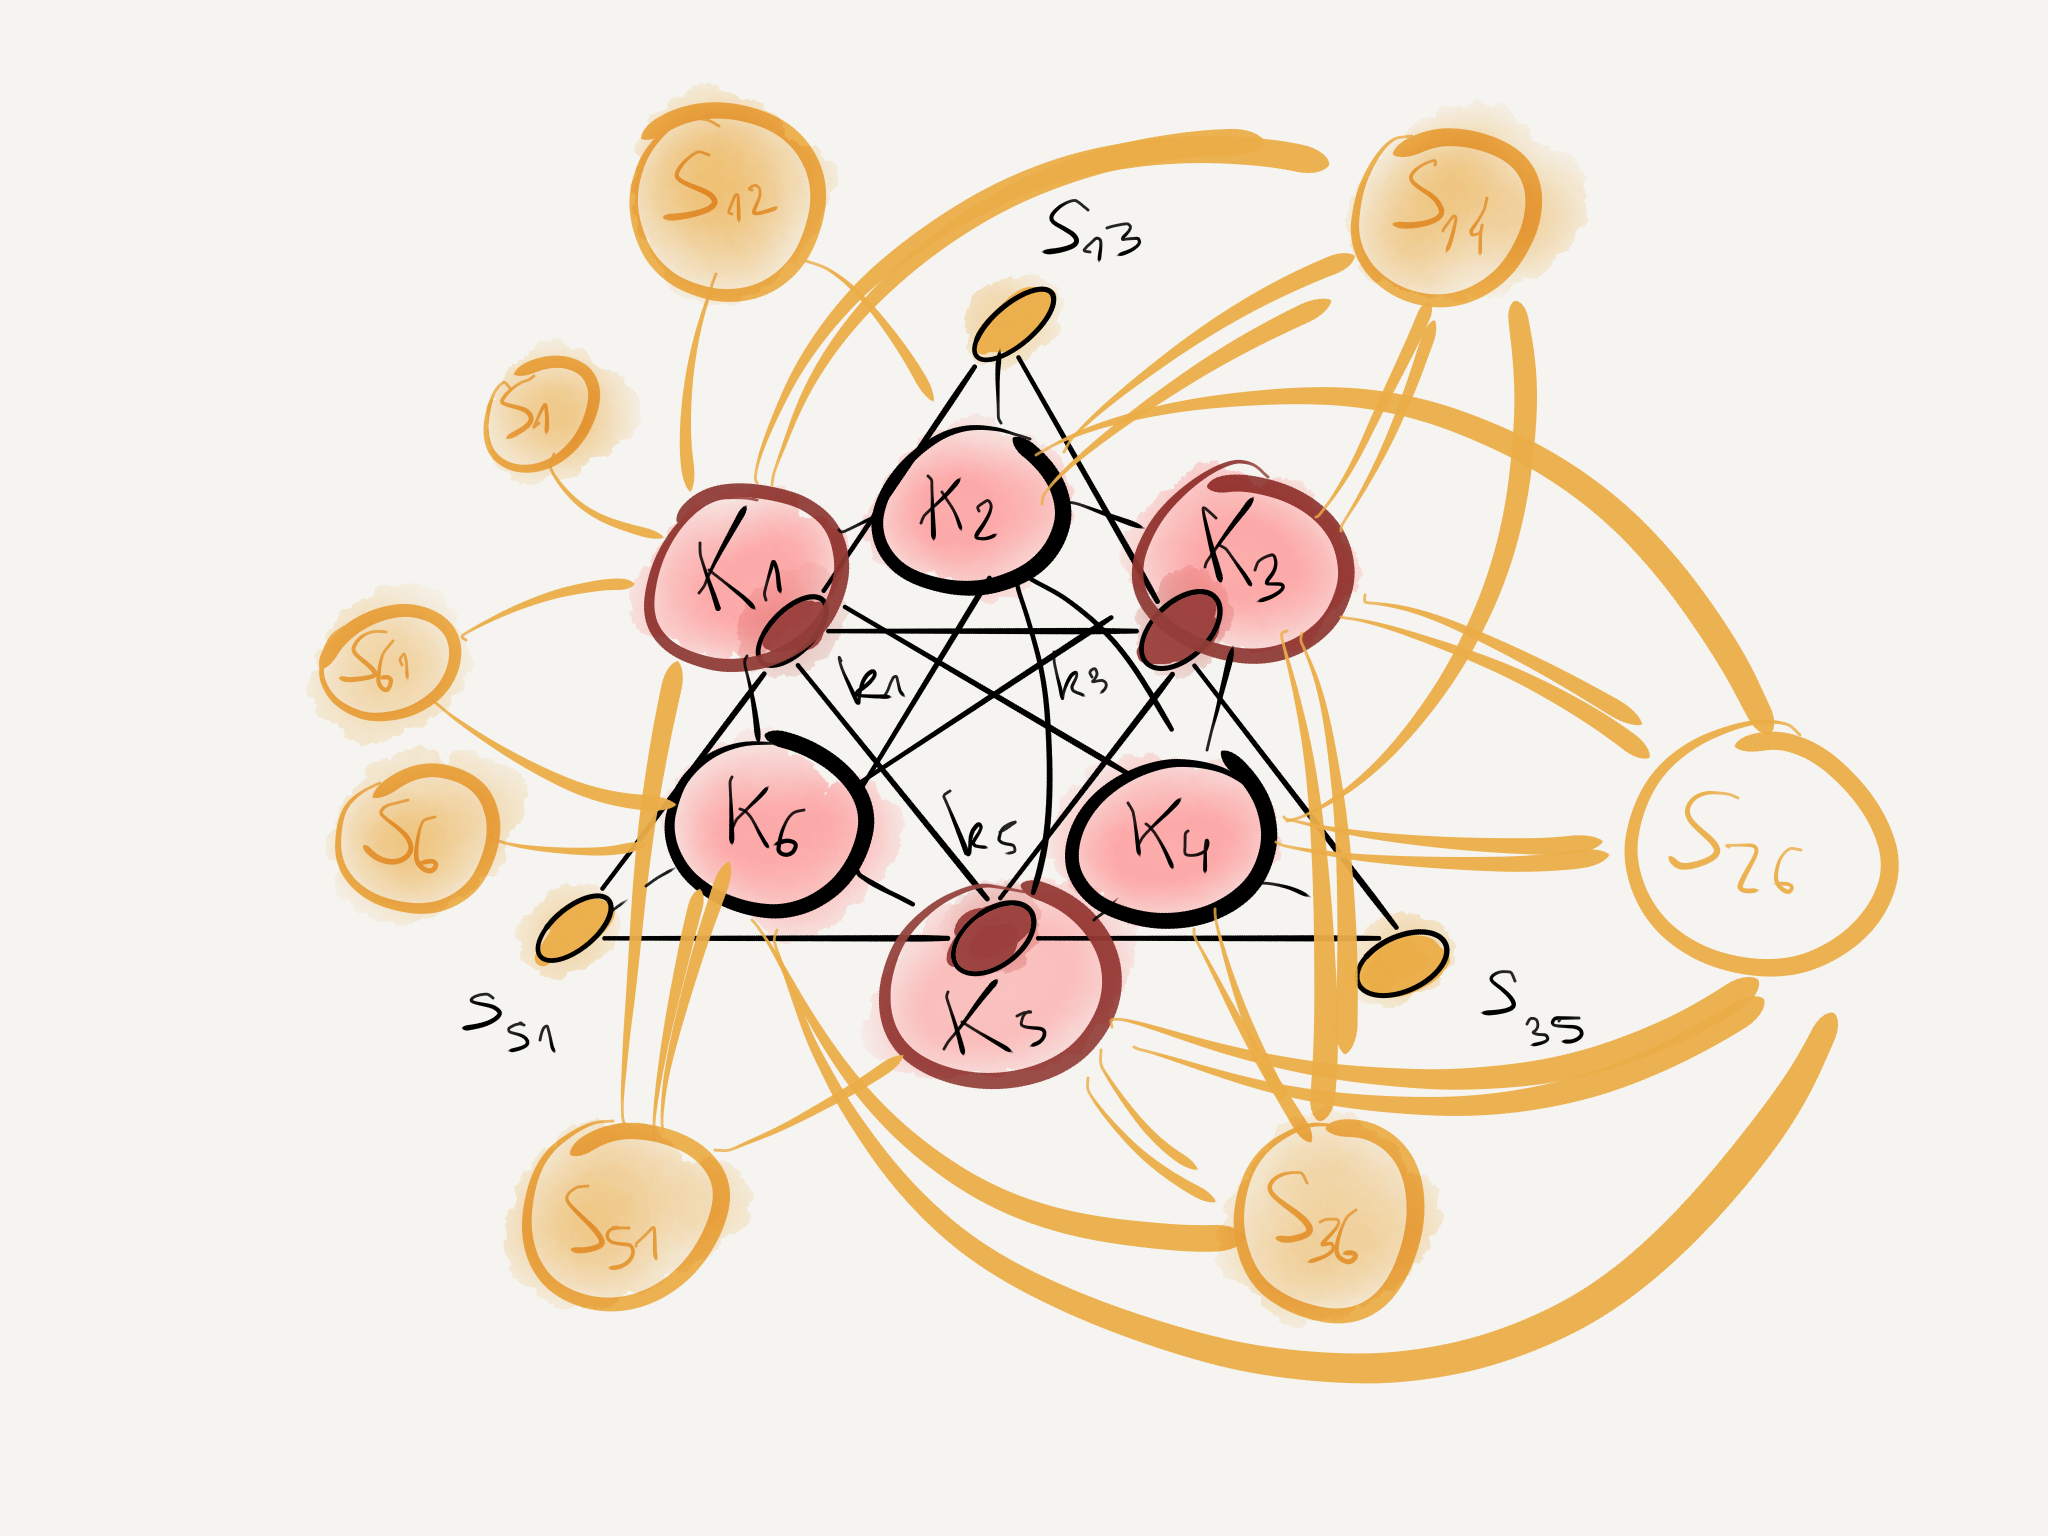
\includegraphics[scale=.15]{tent_ext.png}
	\end{center}
	\caption{Tent $T$ and the split graph $G$ according to the given extensions}
\end{figure}

\subsection{Matrices $\mathbb A_1,\mathbb A_2,\ldots,\mathbb A_6$}

Let $G=(K,S)$ and $T$ as in the previous subsection.

For each $i\in\{1,2,\ldots,6\}$, let $\mathbb A_i$ be a $(0,1)$-matrix having one row for each vertex $s\in S$ such that $s$ belongs to $S_{ij}$ or $S_{ji}$ for some $j\in\{1,2,\ldots,6\}$ and one column for each vertex $k\in K_i$ and such that such that the entry corresponding to row $s$ and column $k$ is $1$ if and only if $s$ is adjacent to $k$ in $G$. For each $j\in\{1,2,\ldots,6\}$, we mark those rows corresponding to vertices of $S_{ji}$ with $L$ and those corresponding to vertices of $S_{ij}$ with $R$.

Moreover, we color some of the rows of $\mathbb A_i$ as follows.
\begin{itemize}
 \item If $i\in\{1,3,5\}$, then we color each row corresponding to a vertex $s\in S_{ij}$ for some $j\in\{1,2,\ldots,6\}-\{i\}$ with color red and each row corresponding to a vertex $s\in S_{ji}$ for some $j\in\{1,2,\ldots,6\}-\{i\}$ with color blue.
 \item If $i\in\{2,4,6\}$, then we color each row corresponding to a vertex $s\in S_{ij}\cup S_{ji}$ for some $j\in\{1,2,\ldots,6\}$ with color red if $j=i+1$ or $j=i-1$ (modulo $6$) and with color blue otherwise.
\end{itemize}

Example:
\[ \mathbb A_3 = \bordermatrix{ & K_3\cr
		S_{34}\ \textbf{R} & \textcolor{red}{\cdots} \cr
                S_{35}\ \textbf{R} & \textcolor{red}{\cdots} \cr
                S_{33}\            & \cdots \cr
                S_{13}\ \textbf{L} & \textcolor{blue}{\cdots} \cr
                S_{23}\ \textbf{L} & \textcolor{blue}{\cdots}}\qquad\qquad
   \mathbb A_4 = \bordermatrix{ & K_4\cr
		S_{34}\ \textbf{L} & \textcolor{red}{\cdots} \cr
                S_{45}\ \textbf{R} & \textcolor{red}{\cdots} \cr
                S_{44}\            & \cdots \cr
                S_{14}\ \textbf{L} & \textcolor{blue}{\cdots} \cr
                S_{64}\ \textbf{L} & \textcolor{blue}{\cdots} \cr
                S_{41}\ \textbf{R} & \textcolor{blue}{\cdots} \cr
                S_{45}\ \textbf{R} & \textcolor{blue}{\cdots}} \]


\begin{figure}[h!]
  \begin{subfigure}[b]{0.5\textwidth}
    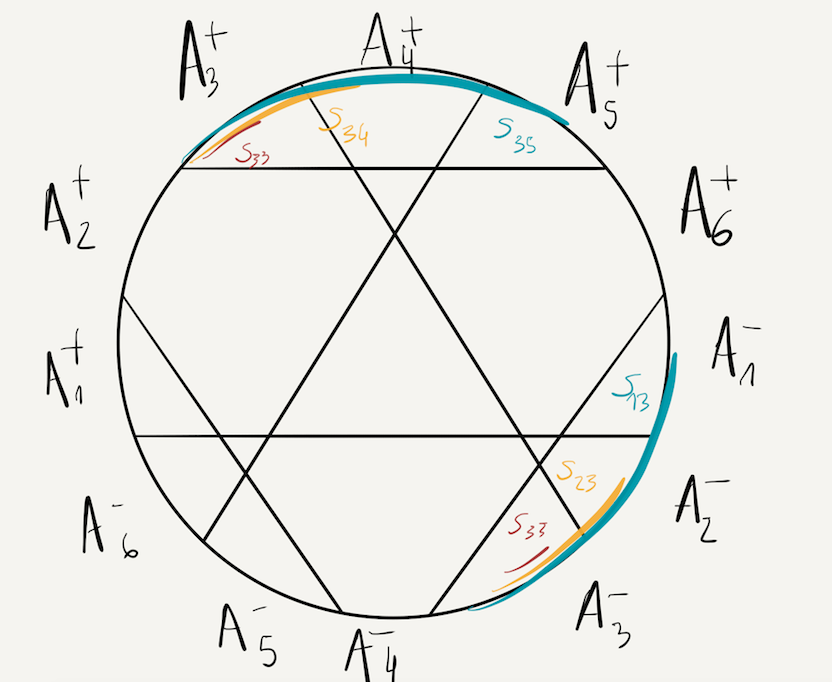
\includegraphics[width=\textwidth]{modelA3.png}
    \caption{$\mathbb{A}_3$}
    \label{fig:modelA3}
  \end{subfigure}
  \hfill
  \begin{subfigure}[b]{0.48\textwidth}
    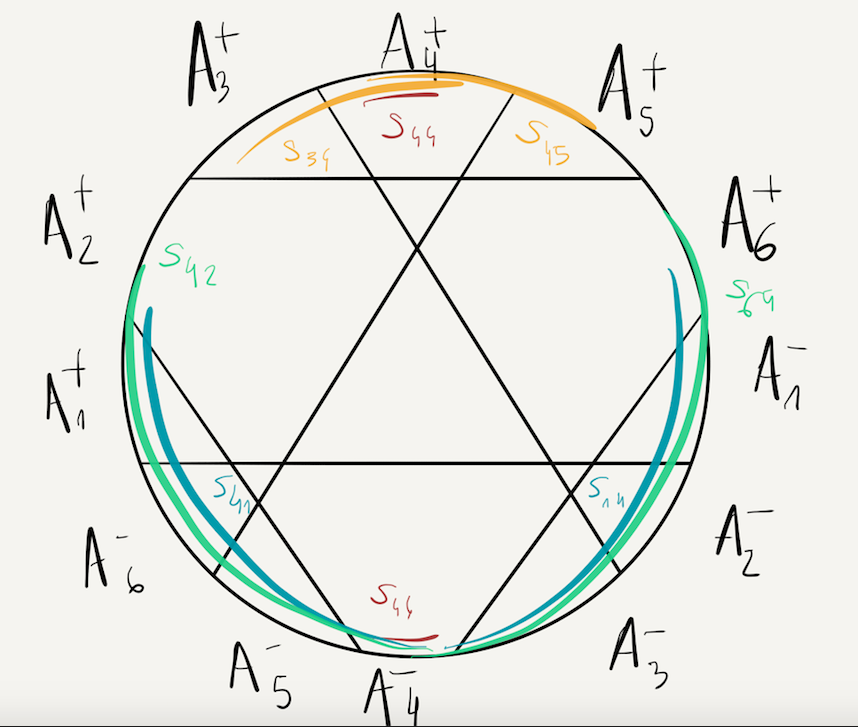
\includegraphics[width=\textwidth]{modelA4.png}
    \caption{$\mathbb{A}_4$}    
    \label{fig:f2}
  \end{subfigure}
  \caption{Sketch model of $G$ with the chords associated to $\mathbb{A}_3$ and $\mathbb{A}_4$, respectively.}
\end{figure}

%\vspace{2mm} 

                
\subsection{circle split equiv. full LRS-sortable}

\begin{lema} 
	If $\mathbb A_i$ is not full LRS-sortable, then $G$ contains one of the following minimal forbidden induced subgraphs for the class of circle graphs: $\ldots$
\end{lema}

\begin{proof}[Proof. (Sketch)] 

Suppose first that $\mathbb A_i$ is not admissible. By Lema~$\cdots$, $\mathbb A_i$ contains some submatrix $D_0,D_1,D_2,D_3$. 

Suppose that $\mathbb A_i$ contains $D_0$. Let $v_0$ and $v_1$ in $S$ be the vertices whose adjacency is represented by the first and second row of $D_0$, respectively, and let $k_{i1}$ and $k_{i2}$ in $K_i$ be the vertices whose adjacency is represented by the second and third column of $D_0$.

%%%????????

Since $v_1$ is an unmarked vertex, then $v_1$ must be in $S_{(i)(i)}$. Moreover, since $v_0$ and $v_1$ are both colored with the same color and $v_0$ is marked, we have to analize each case depending on whether $i$ is even or odd. 
Since the cases are symmetric, we assume without loss of generality that $v_0$ is marked with L.

If $i$ is even, then the possibilities are $v_0 \in S_{(i-1)(i)}, v_1 \in S_{(i)(i)}$, $v_0 \in S_{(i-3)(i)}, v_1 \in S_{(i)(i)}$ and $v_0 \in S_{(i+2)(i)}, v_1 \in S_{(i)(i)}$.
If $i$ is odd, and assuming the even case proven, then the only remaining case is when $v_0 \in S_{(i-2)(i)}, v_1 \in S_{(i)(i)}$.

Case 1.1. $v_0 \in S_{(i-1)(i)}, v_1 \in S_{(i)(i)}$



Para cada una de esas matrices encontrar el subgrafo prohibido inducido de circle en $G$.

Suppose now that $\mathbb A_i$ is admissible but not LR-sortable. Then it contains ... y por cada una de ellas dar el prohibido. (ejemplo: el prohibido de la foto, Mv)\end{proof}

\begin{teo} 
	Let $G=(K,S)$ be a split graph containing an induced tent. Then, $G$ is a circle graph if and only if $\mathbb A_1,\mathbb A_2,\ldots,\mathbb A_6$ are full LRS-sortable.
\end{teo}

\begin{proof}[Sketch.] Necessity is clear by the previous lemma. Suppose now that each of the matrices $\mathbb A_1,\mathbb A_2,\ldots,\mathbb A_6$ are full LRS-sortable. Let $\Pi_i$ be the order of the column in a LR-ordering of $\mathbb A_i$ for each $i\in\{1,2,\ldots,6\}$. Consider the circle divided into twelve pieces as in Figure~.... For each $i\in\{1,2,\ldots,6\}$ and for each vertex $k_i\in K_i$ we place a chord having one end in $A_i^+$ and another in in $A_i^-$ in such a way that the ordering of the endpoints of the chords in $A_i^+$ and $A_i^-$ is $Pi_i$. Acomodar los extremos en $A_i^+$ y $A_i^-$ de las cuerdas correspondientes a los vértices $s\in S_{ij}$ de acuerdo a $\Pi_i$. Mostrar que el modelo resultante es un modelo circle del grafo.\end{proof}

%TODO: Agregar la figura con las 12 partes y completar la demostración.



%Grafo split a particion, a la matriz $\mathbb A_A$, de ahí a las submatrices prohibidas LR plus, y de ahí a los subgrafos prohibidos en el grafo split original.

%Se pasa de las particiones a las matrices, y de las submatrices prohibidas LR al grafo.

%Cómo se pasa de las particiones a las matrices, que son sortable, y entonces a partir de eso armamos el modelo así. Es decir, dar a partir del orden que tengo de la matriz, cómo defino las regiones en el modelo, y etc.





%%%%%%%%%%%%%%%%%%
%%%%%%%%%%%%%%%%%%
%%%%%%%%%%%%%%%%%%
%%%%%%%%%%%%%%%%%%

\begin{thebibliography}{Weibel}

%B

%K
%\bibitem{KK98} T. Kloks, D. Kratsch; \emph{Listing all minimal separators of a graph}, SIAM Journal on Computing, 27, 605--613, 1998.

\end{thebibliography}


\end{document}

